% ============================================================
% Method: the discrepancy-based VAE (Milan's part, ~15 min)
% ============================================================

\begin{frame}{From identifiability to an algorithm}
  \vspace{2ex}
  \begin{itemize}
    \item Non-constructive proofs: how to obtain $\cG$, $U$, $T(I)$?
    \item True $\cG$ is the \textbf{sparsest model compatible with the data}
  \end{itemize}
  \[
    \max_\theta \; \sum_x \log p_\theta(x) \;-\; \lambda\,|\cG_\theta|
  \]
  \centering\small
  penalized likelihood $\;\to\;$ continuous relaxation $\;\to\;$ variational bound (ELBO) $\;\to\;$ \textbf{discrepancy VAE}
  \par\vspace{3ex}\raggedright
  \lbl{Intuition:} ``fit the data with as few causal edges as possible''

  \note{
    ~1 min
    \begin{itemize}
      \item The identifiability proofs tell us the answer is unique, but are not constructive: they do not give a procedure to find $\cG$, $U$ and the targets.
      \item But the proof of Theorem 2 says: the true graph is the SPARSEST model that is compatible with all the data.
      \item Natural idea: penalized maximum likelihood (like GES / BIC scores in causal discovery).
      \item Exact search over DAGs is combinatorial. Instead: relax to a continuous problem, replace the likelihood by a variational lower bound (VAE), and train by gradient descent.
      \item The rest of my part: what has to be added to a standard VAE to make this work.
    \end{itemize}
  }
\end{frame}

% ------------------------------------------------------------
\begin{frame}{Generative model: from VAE to causal VAE}
  \vspace{1ex}
  \centering
  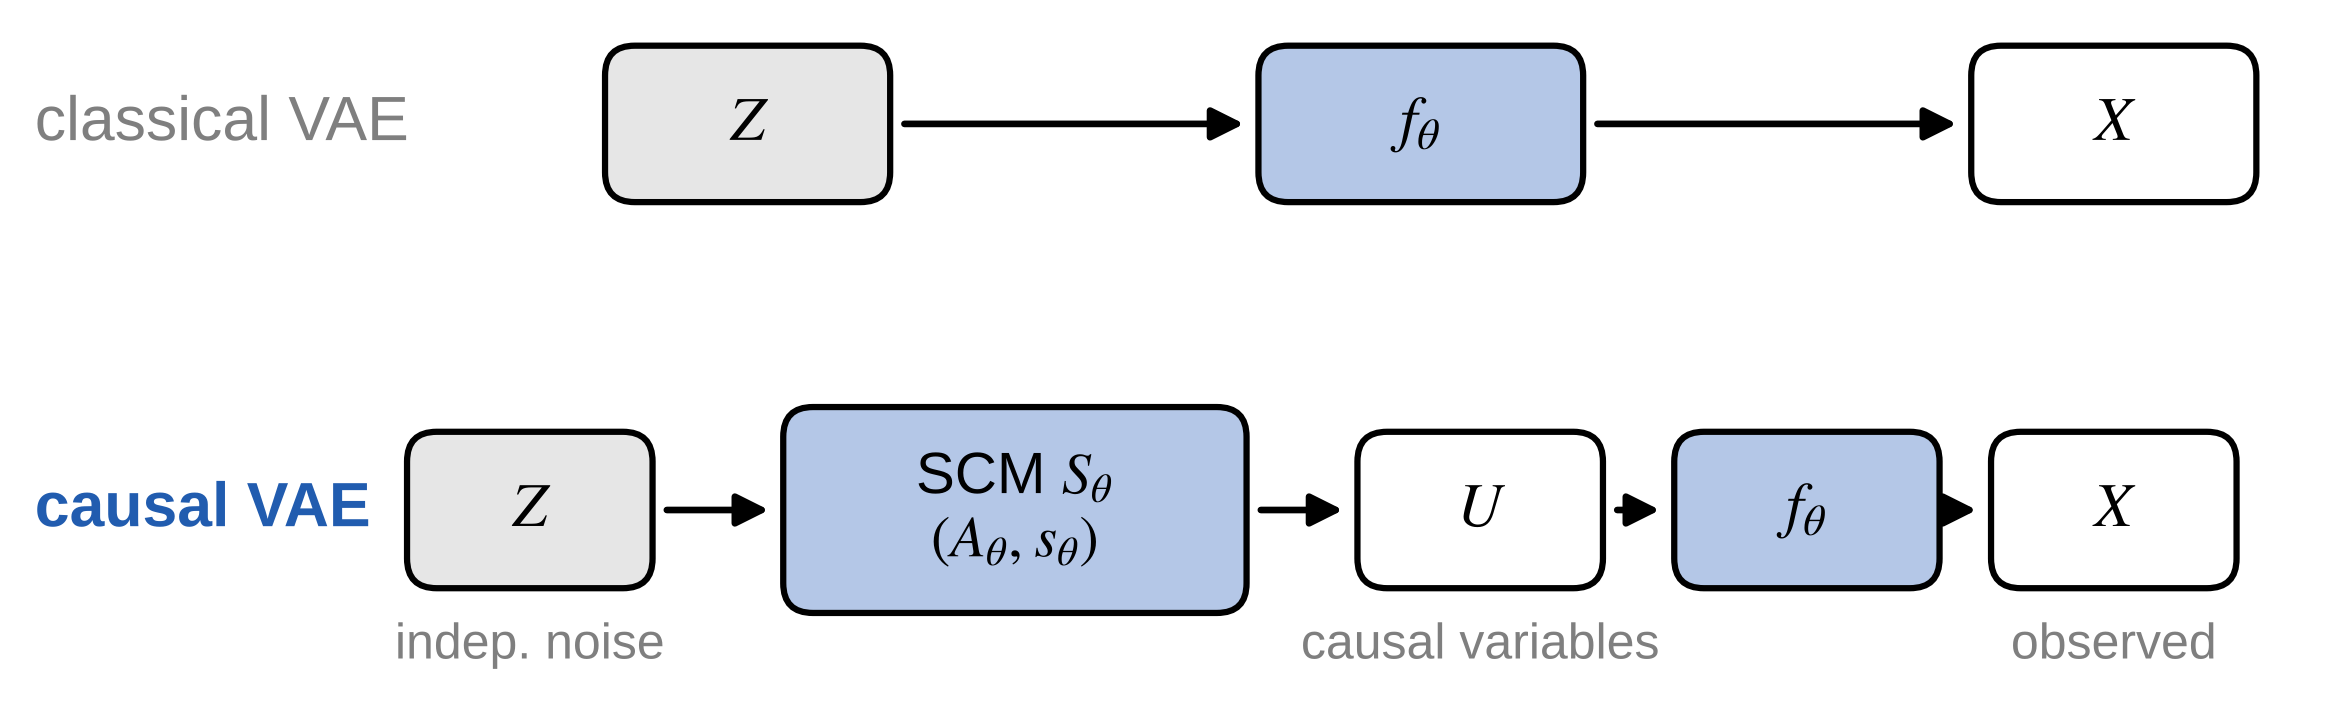
\includegraphics[width=0.78\textwidth]{vae_vs_causal_vae}
  \par\medskip\raggedright
  \renewcommand{\arraystretch}{1.5}
  \begin{tabular}{@{}p{2.6cm}l@{}}
    \textbf{Classical VAE} & $Z \sim \cN(0, I_p), \qquad X \mid Z \sim \cN\big(f_\theta(Z), \sigma^2 I\big)$ \\
    \textbf{Causal VAE} & $U_i = s_{\theta,i}\big(U_{\pa_\cG(i)}, Z_i\big), \quad Z \sim \cN(0, I_p), \qquad X = f_\theta(U)$
  \end{tabular}
  \par\medskip
  \lbl{Intuition:} the encoder still infers independent noise; \textbf{the causal structure lives inside the decoder}

  \note{
    ~1.5 min
    \begin{itemize}
      \item Classical VAE: latent $Z \sim \cN(0,I)$, decoder network $f_\theta$, $X \mid Z \sim \cN(f_\theta(Z), \sigma^2 I)$.
      \item The latent $Z$ has independent coordinates: no causal structure among the latents.
      \item Here: the latents $U$ come from an SCM with DAG $\cG$. Each $U_i$ is a function of its parents and its own exogenous noise $Z_i$. The noise $Z$ is still $\cN(0,I)$.
      \item So the decoder now has two parts: a causal layer (SCM) $Z \to U$, then the mixing $f_\theta: U \to X$.
      \item Key point: the ``standard VAE latent'' is now the exogenous noise $Z$, and the causal variables $U$ are an intermediate layer of the decoder.
    \end{itemize}
  }
\end{frame}

% ------------------------------------------------------------
\begin{frame}{Parametrizing the SCM: a linear causal layer}
  \vspace{1ex}
  \begin{columns}[T]
    \begin{column}{0.6\textwidth}
      \vspace{-2ex}
      \begin{align*}
        U_i &= \textstyle\sum_j (\Ath)_{ij} U_j + Z_i \\
        U &= \Ath U + Z \;\;\Rightarrow\;\; U = (I - \Ath)^{-1} Z =: S_\theta(Z) \\
        X &= f_\theta\big(S_\theta(Z)\big)
      \end{align*}
      WLOG $\bm{A_\theta}$ \textbf{strictly triangular} $\Rightarrow$ always a DAG, $I - \Ath$ invertible
      \[
        (I - \Ath)^{-1} = I + \Ath + \Ath^2 + \dots + \Ath^{p-1}
      \]
    \end{column}
    \begin{column}{0.34\textwidth}
      \centering
      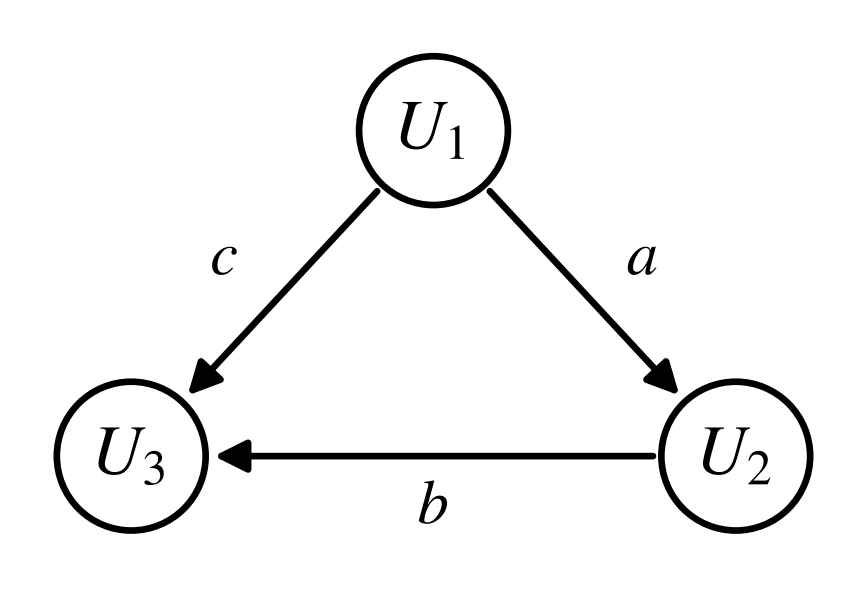
\includegraphics[width=0.8\linewidth]{dag_abc}
      \[
        \Ath = \begin{pmatrix} 0 & 0 & 0 \\ a & 0 & 0 \\ c & b & 0 \end{pmatrix}
      \]
      \[ U_3 = (c + ab) Z_1 + b Z_2 + Z_3 \]
    \end{column}
  \end{columns}
  \vfill
  \lbl{Intuition:} $(I - \Ath)^{-1}$ sums over all directed paths: \textbf{direct} ($c$) + \textbf{indirect} ($ab$) causal effects
  \vspace{2ex}

  \note{
    ~2 min
    \begin{itemize}
      \item In the implementation the SCM is linear with a learnable weighted adjacency matrix $A_\theta$: $(A_\theta)_{ij}$ is the weight of edge $j \to i$.
      \item Solving $U = AU + Z$ gives $U = (I - A)^{-1} Z =: S_\theta(Z)$: the whole SCM is just one matrix multiplication, a linear layer in the decoder.
      \item WLOG $A_\theta$ is strictly triangular (we may order the nodes topologically, since CD-equivalence allows relabelling). The paper says ``upper triangular'' (row-vector convention in the code). Triangular $\Rightarrow$ nilpotent $\Rightarrow$ $I - A$ always invertible, $\det = 1$, and the graph is automatically acyclic. No NOTEARS-style acyclicity constraint needed.
      \item Intuition: Neumann series $(I-A)^{-1} = I + A + \dots + A^{p-1}$. $A^k$ collects all paths of length $k$. So entry $(i,j)$ = sum over all directed paths $j \to \dots \to i$ of products of edge weights = the total causal effect of $Z_j$ on $U_i$.
      \item Example: $U_3 = (c + ab) Z_1 + b Z_2 + Z_3$: $c$ is the direct effect, $ab$ the effect through $U_2$.
      \item The nonlinearity sits in $f_\theta$ (neural net), so a linear SCM costs little expressiveness (App.\ F).
    \end{itemize}
  }
\end{frame}

% ------------------------------------------------------------
\begin{frame}{Observational distribution and the ELBO}
  \vspace{-1ex}
  {\small
  \begin{gather*}
    p_{\theta,\emptyset}(x) = \int p_\theta\big(x \mid U = S_\theta(z)\big)\, p(z)\, dz \\
    q_\phi(z \mid x) = \cN\big(\mu_\phi(x), \diag \sigma^2_\phi(x)\big) \approx p_{\theta,\emptyset}(z \mid x) \\
    \log p_{\theta,\emptyset}(x) \;\geq\; \EE_{q_\phi(Z \mid x)}\big[\log p_{\theta,\emptyset}(x \mid Z)\big] - D_{\KL}\big(q_\phi(Z \mid x) \,\|\, \cN(0, I_p)\big)
  \end{gather*}}
  \vspace{-2ex}
  \begin{columns}[T]
    \begin{column}{0.36\textwidth}
      \textbf{+ sparsity:} $-\lambda \|\Ath\|_1$
      \begin{itemize}
        \item encoder returns noise $\hZ$, not $U$
        \item so far: a standard VAE with a causal layer in the decoder
      \end{itemize}
    \end{column}
    \begin{column}{0.6\textwidth}
      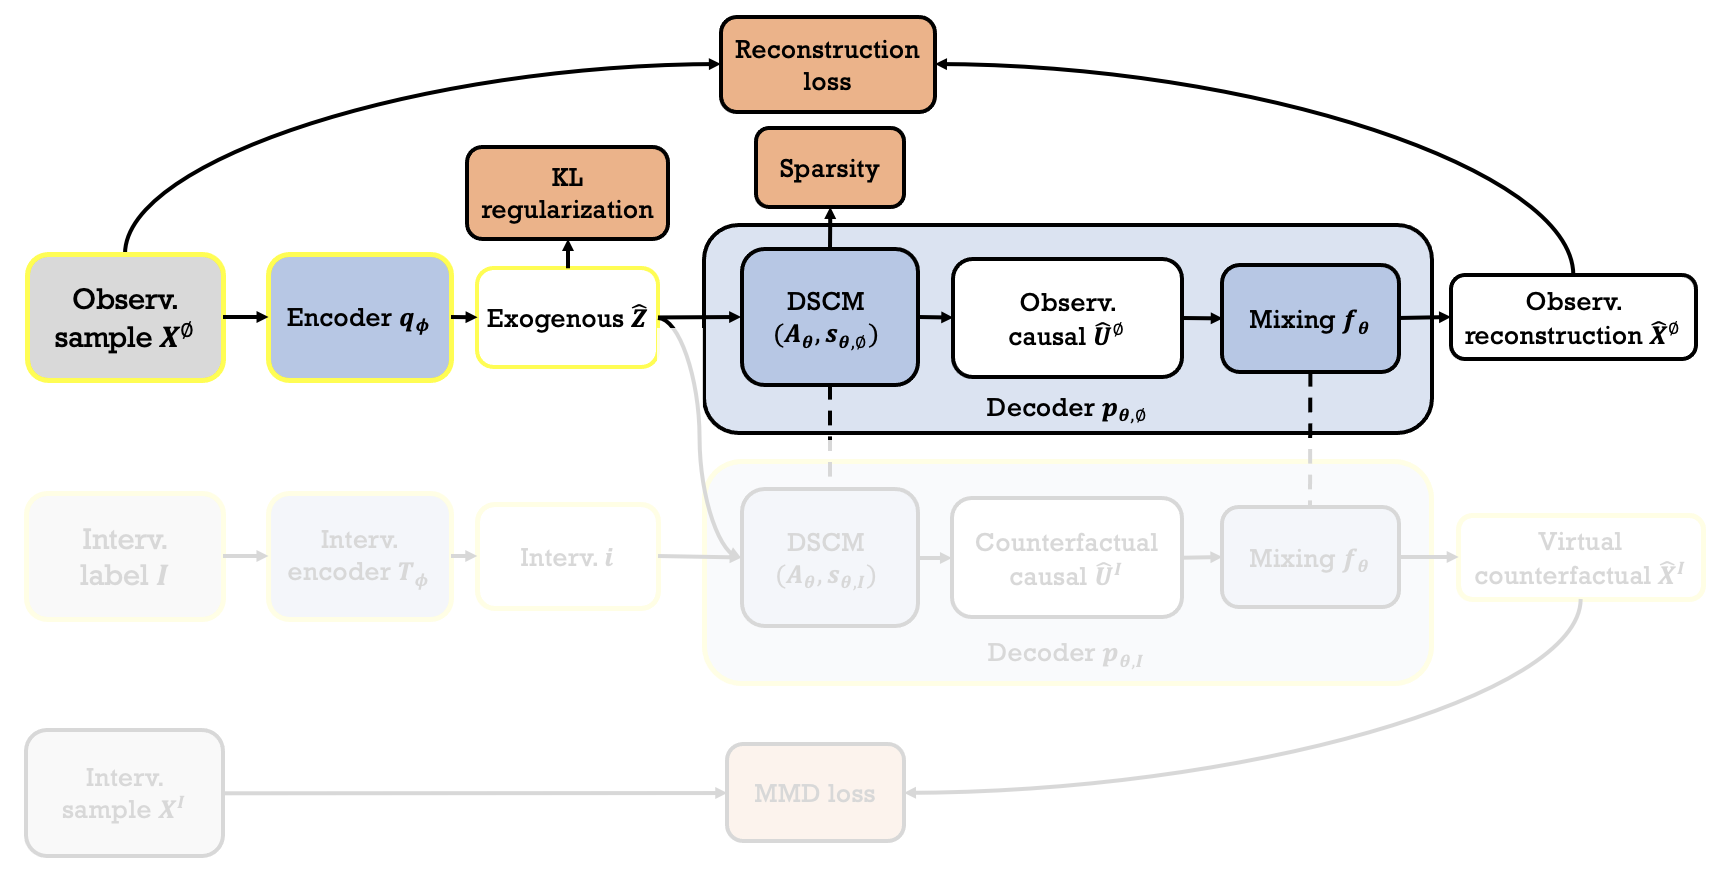
\includegraphics[width=\linewidth]{arch_observational}
    \end{column}
  \end{columns}

  \note{
    ~1.5 min
    \begin{itemize}
      \item The decoder ($Z \sim \cN(0,I)$, $U = S_\theta(Z)$, $X \sim p_\theta(x \mid U)$) induces the observational distribution $p_{\theta,\emptyset}(x)$.
      \item As in every VAE, the posterior $p(z \mid x)$ is intractable, so we introduce an encoder $q_\phi(z \mid x)$ (Gaussian with NN mean and variance) and maximise the ELBO.
      \item Note: the encoder outputs $\hZ$, the noise, not $U$. $\hU = S_\theta(\hZ)$ follows deterministically.
      \item Extra term: L1 penalty on $A_\theta$: the ``sparsest compatible model'' from Theorem 2, relaxed.
      \item In the figure: only the top row is active so far: this is a standard VAE, with a causal layer inside the decoder.
    \end{itemize}
  }
\end{frame}

% ------------------------------------------------------------
\begin{frame}{Interventions in the model}
  \vspace{1ex}
  \begin{columns}[T]
    \begin{column}{0.64\textwidth}
      \begin{gather*}
        U^I_i = s_{\theta,i}\big(U^I_{\pa(i)}, Z_i\big) + a^I\, \mathbf{1}\{T(I) = i\} \\
        U^I = (I - \Ath)^{-1}\big(Z + a^I e_{T(I)}\big), \qquad X^I = f_\theta(U^I)
      \end{gather*}
      \begin{itemize}
        \item same noise $Z$, same mechanisms, same $f_\theta$
        \item only the target is pushed
        \item unknown: target $\bm{T(I)}$ and shift $\bm{a^I}$ $\to$ learn them
      \end{itemize}
    \end{column}
    \begin{column}{0.3\textwidth}
      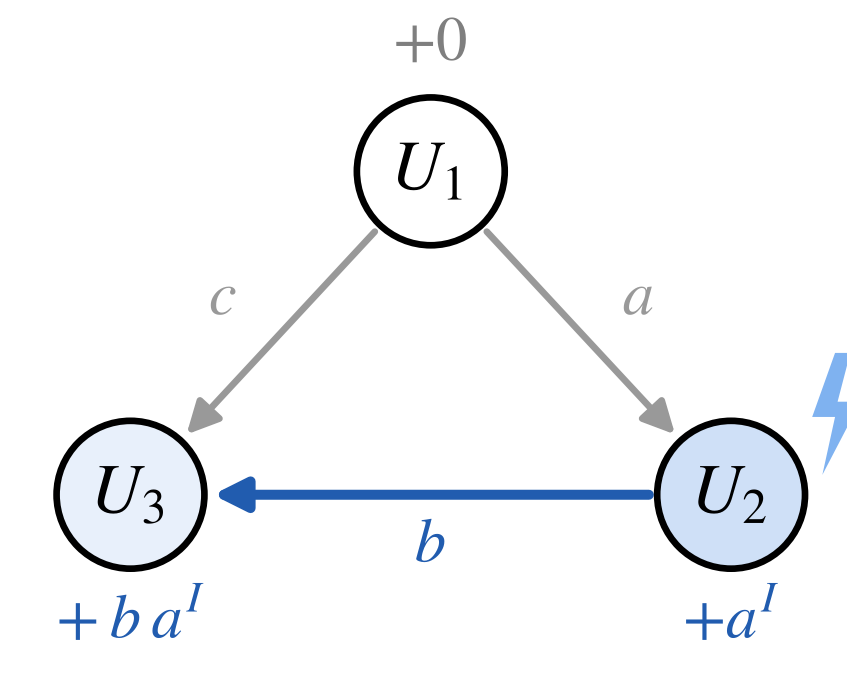
\includegraphics[width=\linewidth]{dag_shift}
    \end{column}
  \end{columns}

  \note{
    ~1.5 min
    \begin{itemize}
      \item Interventions are modelled as shift interventions: intervention $I$ has one target $T(I) \in [p]$ and a shift $a^I$. The target node gets $a^I$ added to its mechanism.
      \item This is soft: $U_T$ still depends on its parents.
      \item Everything else stays the same: the same noise $Z$, the other mechanisms, and the same mixing $f_\theta$. Modularity / ``sparse mechanism shift''.
      \item Linear case: $U^I = (I - A)^{-1}(Z + a^I e_T)$. The difference to the observational $U$ is $a^I$ times column $T$ of the path matrix: the shift propagates exactly to the descendants of $T$.
      \item Example: shifting $U_2$ shifts $U_3$ by $b a^I$, and $U_1$ not at all.
      \item Problem: the intervention label $I$ is known (we know which CRISPR guide was used), but which latent node it hits, $T(I)$, and how strongly, $a^I$, are unknown. They must be learned.
    \end{itemize}
  }
\end{frame}

% ------------------------------------------------------------
\begin{frame}{Learning the intervention: target and shift encoder}
  \vspace{1ex}
  \begin{columns}[T]
    \begin{column}{0.48\textwidth}
      \vspace{-2ex}
      \begin{gather*}
        I \;\mapsto\; \big(T_\phi(I),\, a_\phi(I)\big) \in \Delta^{p-1} \times \R \\
        T_\phi(I)_i = \frac{\exp\big(t \cdot \tilde T_\phi(I)_i\big)}{\sum_{j=1}^p \exp\big(t \cdot \tilde T_\phi(I)_j\big)} \\
        \Ucf^I = (I - \Ath)^{-1}\big(Z + a_\phi(I)\, T_\phi(I)\big)
      \end{gather*}
    \end{column}
    \begin{column}{0.48\textwidth}
      \begin{itemize}
        \item ``which node?'' is discrete $\to$ \textbf{softmax relaxation}
        \item annealing: $\bm{t = 1}$ first half, then $\uparrow$ to $\bm{100}$
        \item test time: $\approx$ one-hot target
      \end{itemize}
    \end{column}
  \end{columns}
  \par\smallskip\centering
  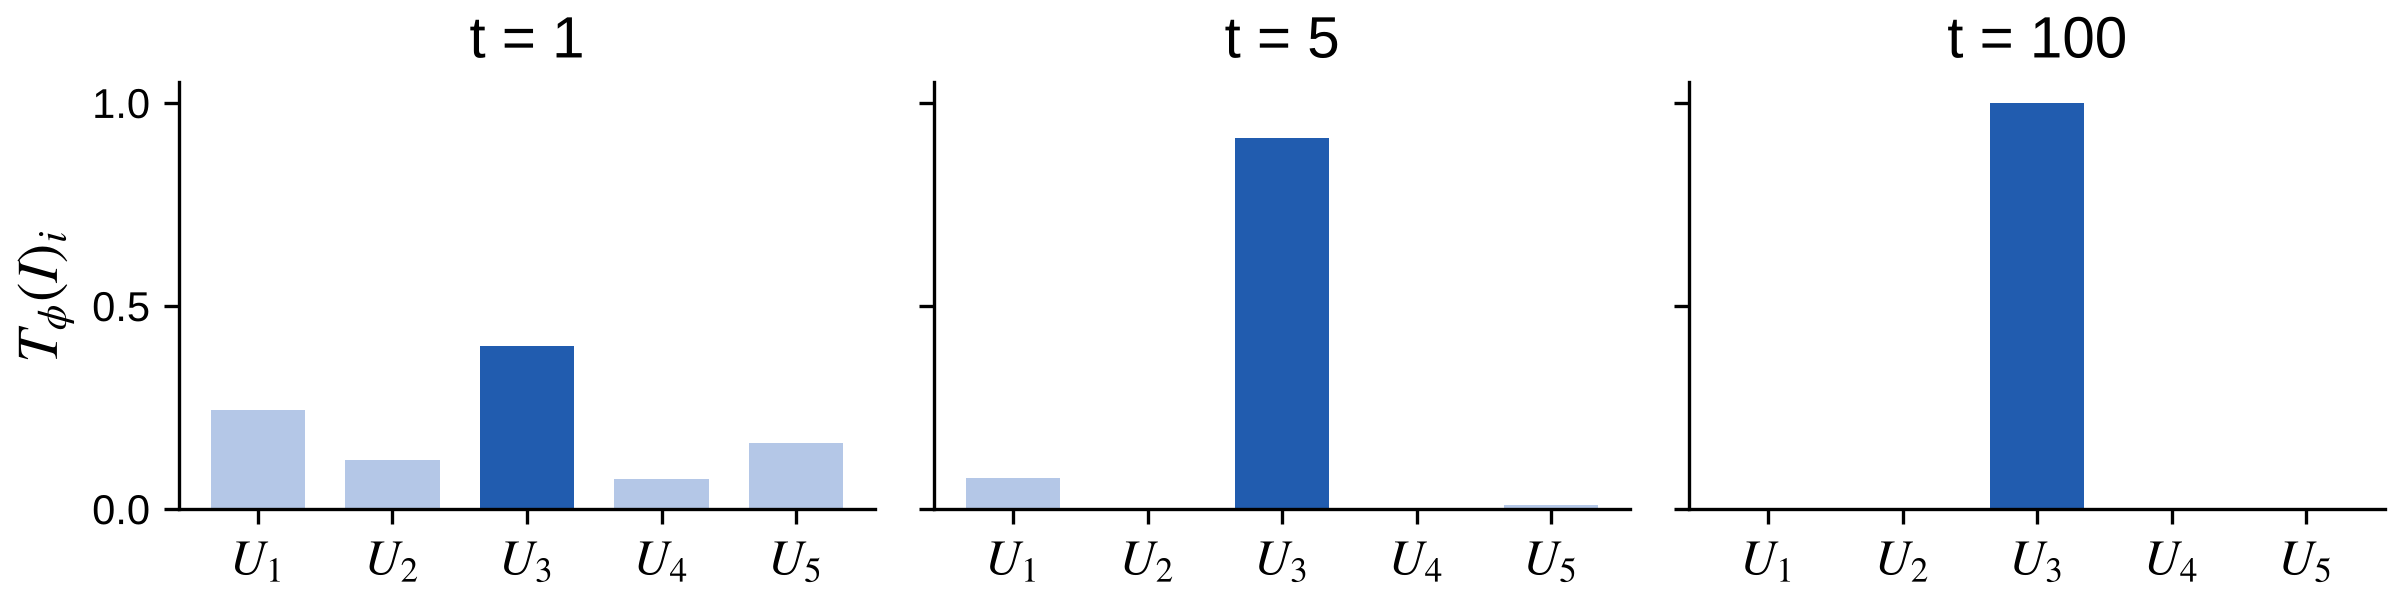
\includegraphics[width=0.66\textwidth]{softmax_annealing}
  \par\smallskip\raggedright
  \lbl{Intuition:} \textbf{start soft} (explore all candidate targets), \textbf{end hard} (one target per intervention)

  \note{
    ~1.5 min
    \begin{itemize}
      \item A second encoder maps the intervention label $I$ (just a one-hot over the $K$ interventions) to a predicted target $T_\phi(I)$ and shift $a_\phi(I)$.
      \item ``Which latent node?'' is a discrete choice, so not differentiable. Relax it: $T_\phi(I)$ is a softmax over the $p$ nodes, i.e.\ a point in the simplex. The shift is then spread over nodes according to these weights.
      \item Temperature $t$ controls how peaked the softmax is. $t = 1$: soft, the model can explore several targets. $t$ large: essentially one-hot.
      \item Annealing schedule (App.\ F): $t = 1$ for the first half of training, then linearly increased to $t_{\max} = 100$; at test time large $t$ $\to$ one-hot target.
      \item Intuition: start soft so gradients flow to all candidate nodes, end hard so each intervention has a single target, as the theory assumes.
    \end{itemize}
  }
\end{frame}

% ------------------------------------------------------------
\begin{frame}{The main trick: virtual counterfactuals}
  \vspace{-1ex}
  \[
    X \sim \cD \;\to\; \hZ \sim q_\phi(\cdot \mid X) \;\to\; \Ucf^I = S_\theta\big(\hZ + \hat a^I \widehat T^I\big) \;\to\; \Xcf^I = f_\theta\big(\Ucf^I\big)
  \]
  \begin{columns}[T]
    \begin{column}{0.36\textwidth}
      \[ \{\Xcf^I\} \overset{?}{\approx} \{X^I\} \sim \cD^I \]
      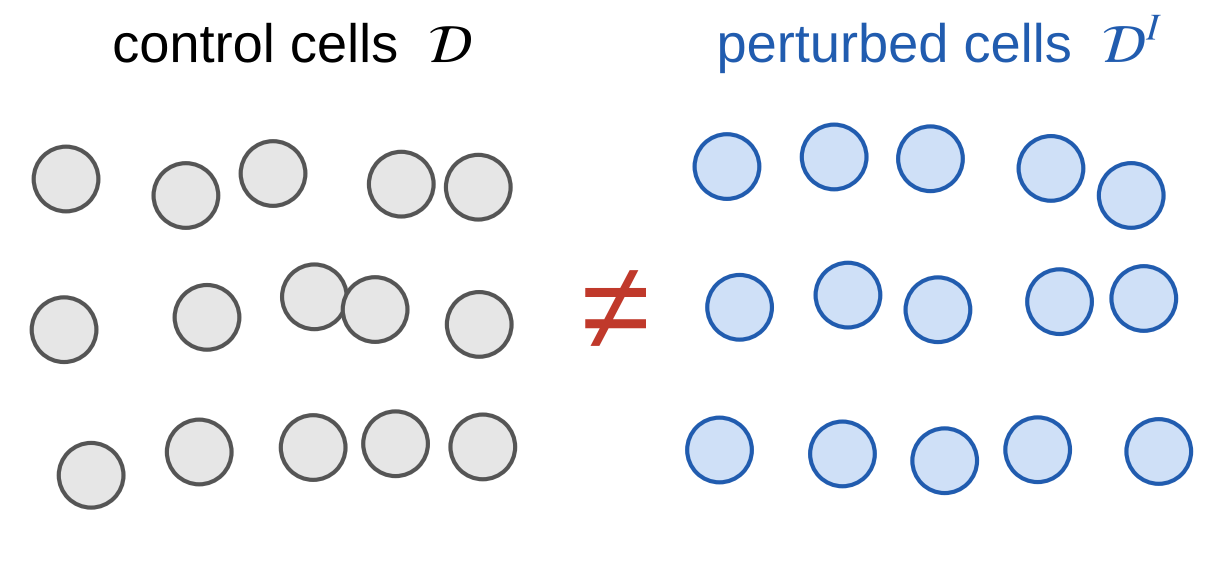
\includegraphics[width=\linewidth]{unpaired}
      \par\medskip
      \lbl{Intuition:} ``what would \textbf{this} cell look like if it had been perturbed?''
    \end{column}
    \begin{column}{0.6\textwidth}
      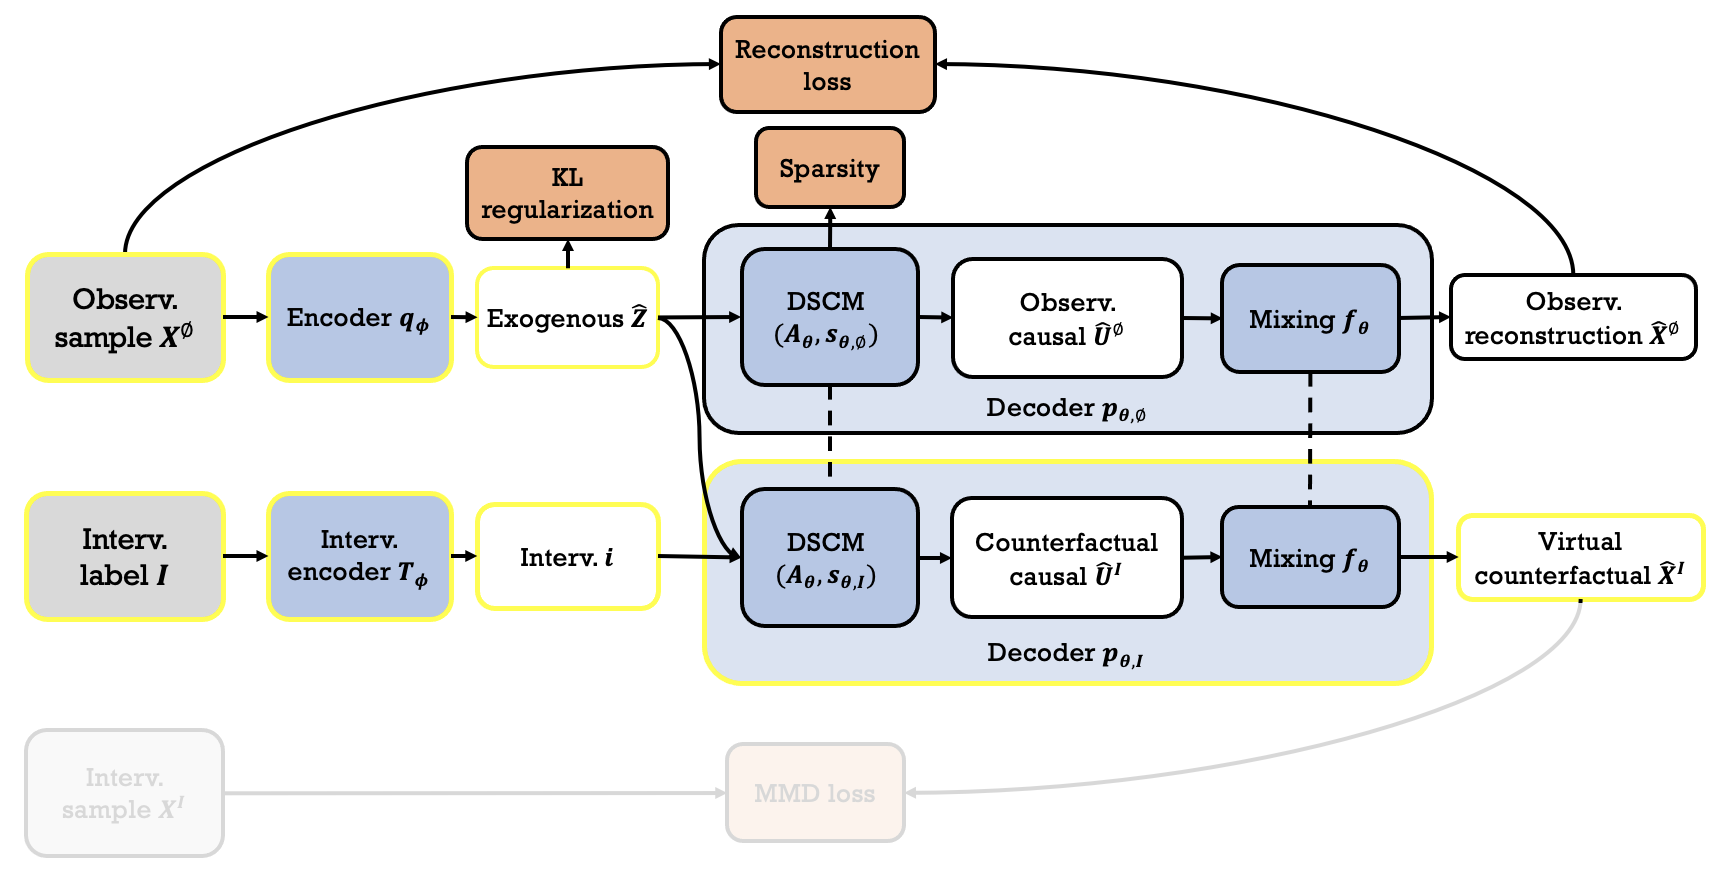
\includegraphics[width=\linewidth]{arch_counterfactual}
    \end{column}
  \end{columns}

  \note{
    ~2 min
    \begin{itemize}
      \item Interventional samples $X^I$ are NOT passed through the encoder $q_\phi$.
      \item Instead, for each observational sample $X$ we ask: what would this cell have looked like had it received intervention $I$?
      \item Encode $X$ to get its noise $\hZ$, apply the predicted intervention $(\hat T, \hat a)$ in the causal layer, decode with the same $f_\theta$: $\Xcf^I$. This is the highlighted path in the paper's figure.
      \item We cannot compare $\Xcf^I$ to ``its'' real counterpart: there is no pairing (each cell measured once). But we can compare the DISTRIBUTION of virtual counterfactuals with the distribution of real interventional samples in $\cD^I$.
      \item Why not just encode $X^I$? Then the encoder could absorb the intervention into $Z$, and the causal layer and target would learn nothing. Forcing the same noise distribution means the change between $\cD$ and $\cD^I$ must be explained by a single shift in the causal layer. That is exactly the structure the theory uses.
    \end{itemize}
  }
\end{frame}

% ------------------------------------------------------------
\begin{frame}{Comparing distributions: MMD}
  \vspace{-1ex}
  \[
    \MMD(P,Q) = \sup_{\|g\|_\cH \leq 1} \EE_P[g(X)] - \EE_Q[g(Y)] = \|\mu_P - \mu_Q\|_\cH
  \]
  \begin{columns}[T]
    \begin{column}{0.5\textwidth}
      \vspace{-3ex}
      \begin{gather*}
        \MMD^2 = \EE k(X,X') + \EE k(Y,Y') - 2\,\EE k(X,Y) \\
        k(x,y) = \textstyle\sum_m \exp\big(-\|x - y\|^2 / 2\sigma_m^2\big)
      \end{gather*}
    \end{column}
    \begin{column}{0.44\textwidth}
      \begin{itemize}
        \item \textbf{characteristic} kernel: $\MMD = 0 \Leftrightarrow P = Q$
        \item \textbf{closed form}, no adversary
      \end{itemize}
    \end{column}
  \end{columns}
  \par\centering
  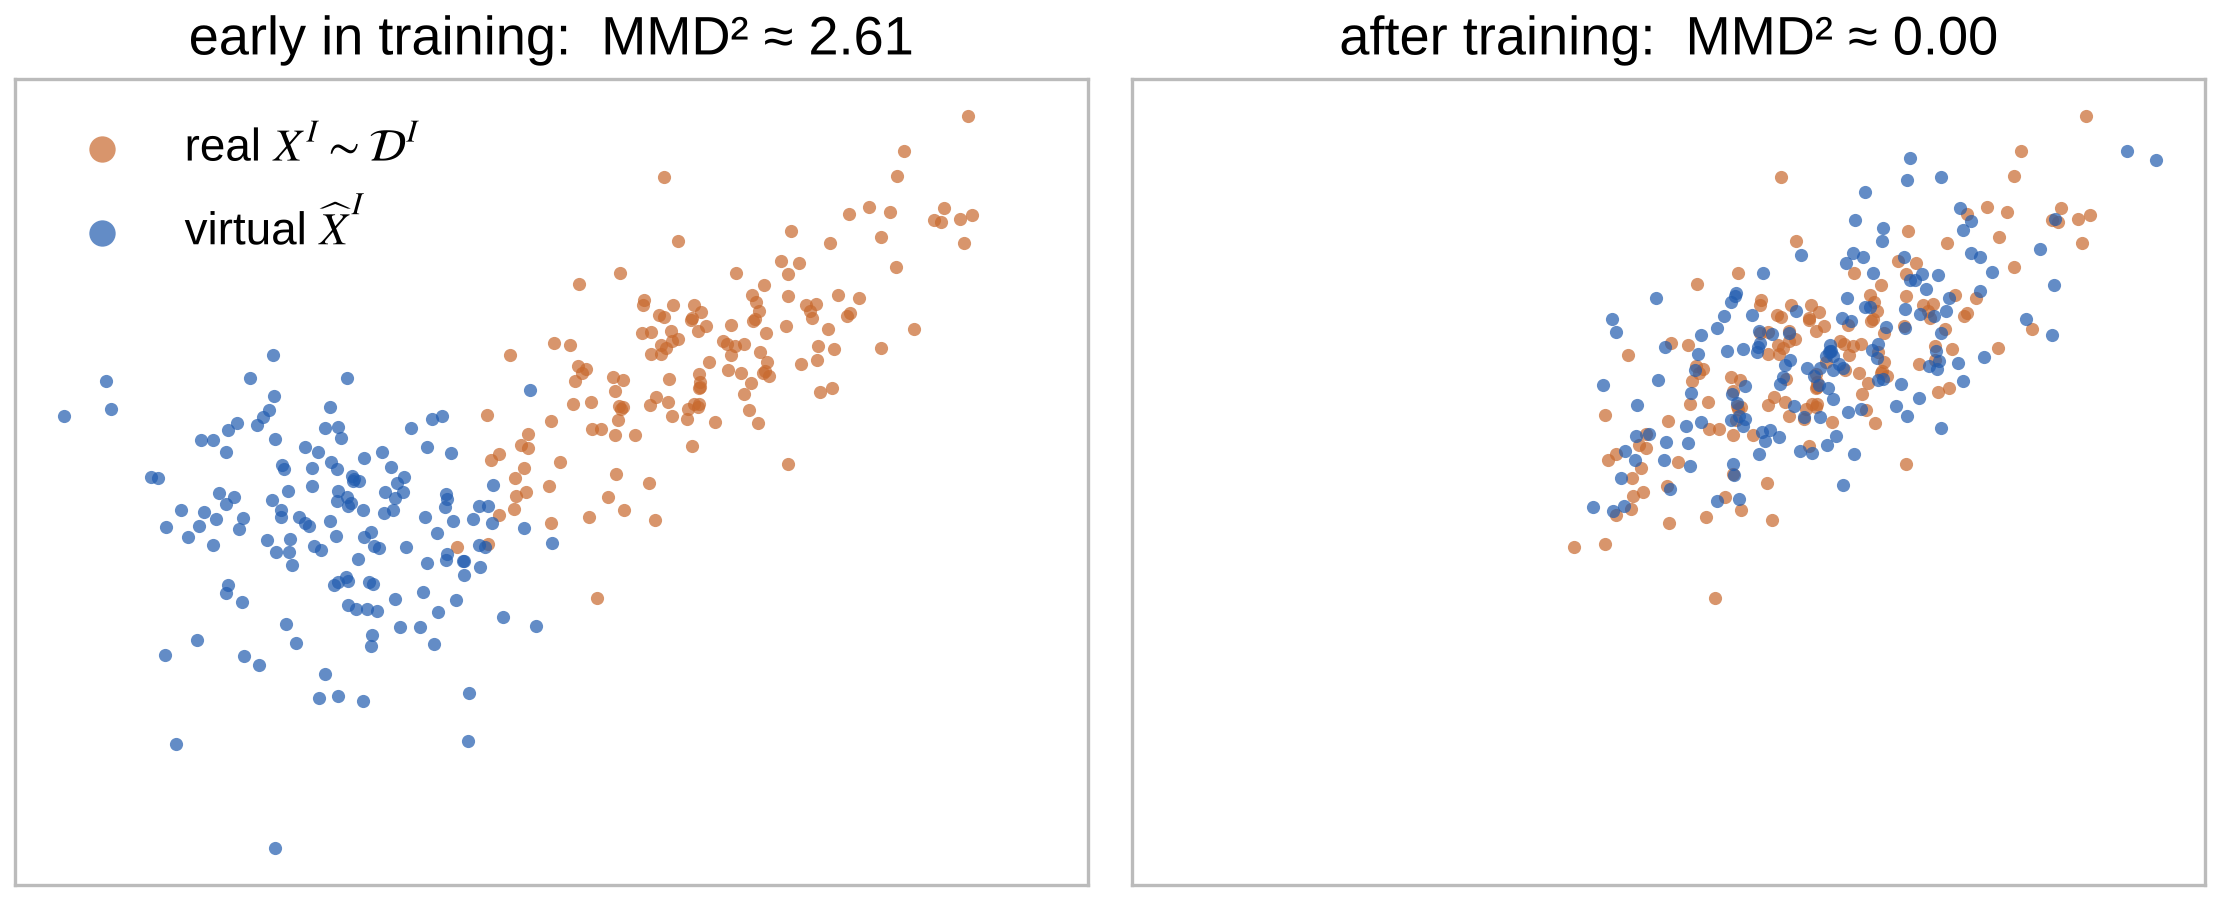
\includegraphics[width=0.6\textwidth]{mmd_clouds}

  \note{
    ~1.5 min
    \begin{itemize}
      \item We need a distance between two sample sets: virtual counterfactuals vs real interventional samples.
      \item MMD: largest difference in expectation over test functions $g$ in the unit ball of an RKHS. By the reproducing property this equals the RKHS distance between the kernel mean embeddings $\mu_P$ and $\mu_Q$.
      \item Empirically: average within-group kernel similarities minus twice the cross-group similarity (unbiased U-statistic, App.\ C.1).
      \item Gaussian kernel is characteristic: $\MMD = 0$ iff $P = Q$, so it compares all moments at once.
      \item Closed form, no adversary: unlike a GAN discriminator there is no min-max game, so training is stable.
      \item Implementation: mixture of 10 Gaussian kernels with dyadically spaced widths (avoids vanishing gradients).
      \item Picture: early in training the virtual cloud is in the wrong place, high MMD; after training they overlap, $\MMD \approx 0$.
    \end{itemize}
  }
\end{frame}

% ------------------------------------------------------------
\begin{frame}{Bringing it all together}
  \vspace{-1ex}
  \centering
  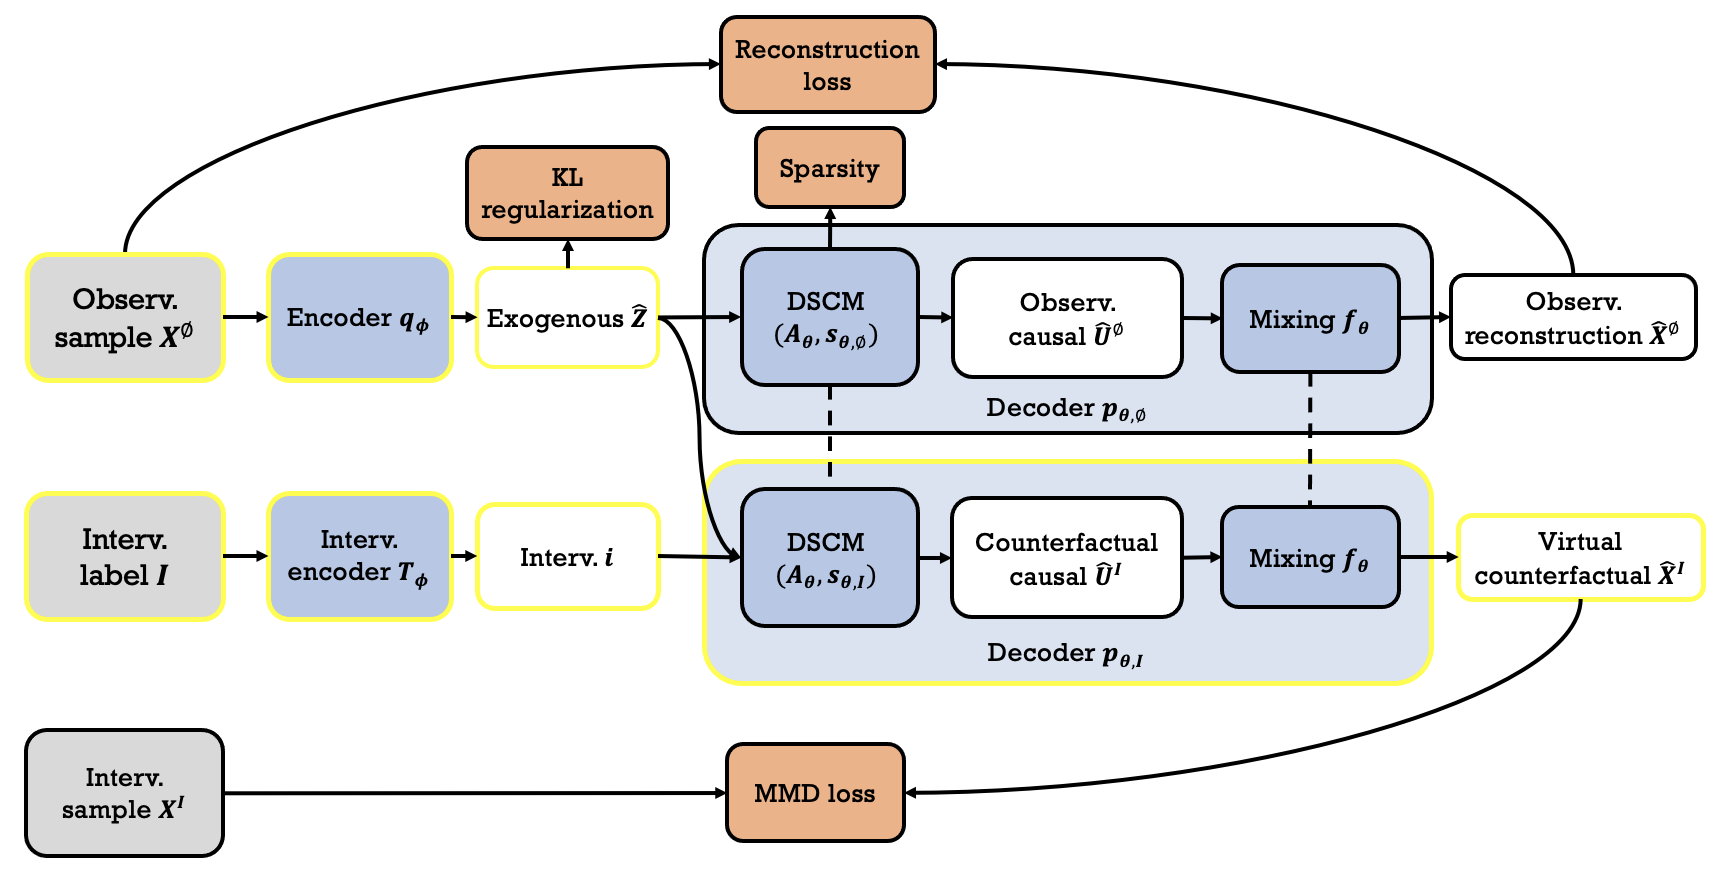
\includegraphics[width=0.62\textwidth]{arch_full}
  {\small
  \[
    \cL = \EE_{X \sim \cD}\Big[\EE_{q_\phi} \log p_{\theta,\emptyset}(X \mid Z) - \beta D_{\KL}(q_\phi \,\|\, p_Z)\Big]
      - \alpha \sum_{k=1}^K \MMD\big(\Xcf^{I_k}, X^{I_k}\big) - \lambda \|\Ath\|_1
  \]}
  \vspace{-1ex}
  {\footnotesize $\beta, \alpha$: warm-up $0 \to 1$ \qquad $\lambda = 0.1$ \qquad shared $\Ath$, $f_\theta$ across rows (dashed)}

  \note{
    ~1.5 min. Walk through the figure once more:
    \begin{itemize}
      \item Top row: observational sample $\to$ encoder $\to$ noise $\hZ$ $\to$ causal layer $(A, s)$ $\to$ $\hU$ $\to$ $f_\theta$ $\to$ reconstruction. Losses: reconstruction, KL, sparsity.
      \item Middle row: intervention label $\to$ intervention encoder $\to$ target/shift; same $\hZ$ goes through the intervened causal layer and the SAME $f_\theta$ $\to$ virtual counterfactual.
      \item Bottom: virtual counterfactuals vs real interventional samples $\to$ MMD loss.
      \item Dashed lines: shared modules (same $A_\theta$, same $f_\theta$).
      \item Loss (maximised): ELBO terms, MMD term, sparsity.
      \item Schedules: $\beta$ and $\alpha$ start at 0 and are warmed up to 1 (KL and MMD switched on gradually); $\lambda = 0.1$. Adam, lr $10^{-3}$, 100 epochs, $<45$ min on one GPU.
      \item Note: eq.\ (3) in the paper has $\beta$ attached to the wrong term; App.\ F makes clear $\beta$ multiplies the KL.
    \end{itemize}
  }
\end{frame}

% ------------------------------------------------------------
\begin{frame}{Why should this work?}
  \vspace{2ex}
  \begin{itemize}
    \item \textbf{Lower bound:} loss $\leq$ paired-data log-likelihood (App.\ D)
    \item \textbf{Consistent:} infinite data $\Rightarrow$ recovers the model up to CD-equivalence (App.\ E)
    \item \textbf{Extrapolation:} combine learned shifts to predict unseen double perturbations
  \end{itemize}
  \[
    \Ucf^{\{I,J\}} = (I - \Ath)^{-1}\big(Z + a^I e_{T(I)} + a^J e_{T(J)}\big)
  \]
  \sep
  \textbf{Caveat:} linear SCM + neural-net decoder lie outside Assumptions 1--2: the theory \textbf{motivates} the method, it does not cover it exactly

  \note{
    ~1 min
    \begin{itemize}
      \item App.\ D: the unpaired loss is a lower bound of the paired-data log-likelihood we would optimise if we had true counterfactual pairs.
      \item App.\ E: consistency. With infinite data and under the conditions of Theorem 2, the optimum recovers the generative process (up to CD-equivalence).
      \item Bonus: because interventions are explicit shifts in the causal layer, we can combine them: predict unseen double perturbations by adding both shifts. The paper evaluates this on the double-gene perturbations.
      \item Honest caveat: the implemented model uses a linear SCM and a neural network $f_\theta$. Linear SCMs violate Assumption 2 (linear interventional faithfulness), and $f_\theta$ is not a polynomial (Assumption 1). So the guarantees motivate the method rather than cover the exact model trained.
    \end{itemize}
  }
\end{frame}
